% Options for packages loaded elsewhere
\PassOptionsToPackage{unicode}{hyperref}
\PassOptionsToPackage{hyphens}{url}
%
\documentclass[
]{article}
\usepackage{amsmath,amssymb}
\usepackage{lmodern}
\usepackage{ifxetex,ifluatex}
\ifnum 0\ifxetex 1\fi\ifluatex 1\fi=0 % if pdftex
  \usepackage[T1]{fontenc}
  \usepackage[utf8]{inputenc}
  \usepackage{textcomp} % provide euro and other symbols
\else % if luatex or xetex
  \usepackage{unicode-math}
  \defaultfontfeatures{Scale=MatchLowercase}
  \defaultfontfeatures[\rmfamily]{Ligatures=TeX,Scale=1}
\fi
% Use upquote if available, for straight quotes in verbatim environments
\IfFileExists{upquote.sty}{\usepackage{upquote}}{}
\IfFileExists{microtype.sty}{% use microtype if available
  \usepackage[]{microtype}
  \UseMicrotypeSet[protrusion]{basicmath} % disable protrusion for tt fonts
}{}
\makeatletter
\@ifundefined{KOMAClassName}{% if non-KOMA class
  \IfFileExists{parskip.sty}{%
    \usepackage{parskip}
  }{% else
    \setlength{\parindent}{0pt}
    \setlength{\parskip}{6pt plus 2pt minus 1pt}}
}{% if KOMA class
  \KOMAoptions{parskip=half}}
\makeatother
\usepackage{xcolor}
\IfFileExists{xurl.sty}{\usepackage{xurl}}{} % add URL line breaks if available
\IfFileExists{bookmark.sty}{\usepackage{bookmark}}{\usepackage{hyperref}}
\hypersetup{
  pdftitle={The importance of uncertainty in contact patterns},
  hidelinks,
  pdfcreator={LaTeX via pandoc}}
\urlstyle{same} % disable monospaced font for URLs
\usepackage[margin=1in]{geometry}
\usepackage{color}
\usepackage{fancyvrb}
\newcommand{\VerbBar}{|}
\newcommand{\VERB}{\Verb[commandchars=\\\{\}]}
\DefineVerbatimEnvironment{Highlighting}{Verbatim}{commandchars=\\\{\}}
% Add ',fontsize=\small' for more characters per line
\usepackage{framed}
\definecolor{shadecolor}{RGB}{248,248,248}
\newenvironment{Shaded}{\begin{snugshade}}{\end{snugshade}}
\newcommand{\AlertTok}[1]{\textcolor[rgb]{0.94,0.16,0.16}{#1}}
\newcommand{\AnnotationTok}[1]{\textcolor[rgb]{0.56,0.35,0.01}{\textbf{\textit{#1}}}}
\newcommand{\AttributeTok}[1]{\textcolor[rgb]{0.77,0.63,0.00}{#1}}
\newcommand{\BaseNTok}[1]{\textcolor[rgb]{0.00,0.00,0.81}{#1}}
\newcommand{\BuiltInTok}[1]{#1}
\newcommand{\CharTok}[1]{\textcolor[rgb]{0.31,0.60,0.02}{#1}}
\newcommand{\CommentTok}[1]{\textcolor[rgb]{0.56,0.35,0.01}{\textit{#1}}}
\newcommand{\CommentVarTok}[1]{\textcolor[rgb]{0.56,0.35,0.01}{\textbf{\textit{#1}}}}
\newcommand{\ConstantTok}[1]{\textcolor[rgb]{0.00,0.00,0.00}{#1}}
\newcommand{\ControlFlowTok}[1]{\textcolor[rgb]{0.13,0.29,0.53}{\textbf{#1}}}
\newcommand{\DataTypeTok}[1]{\textcolor[rgb]{0.13,0.29,0.53}{#1}}
\newcommand{\DecValTok}[1]{\textcolor[rgb]{0.00,0.00,0.81}{#1}}
\newcommand{\DocumentationTok}[1]{\textcolor[rgb]{0.56,0.35,0.01}{\textbf{\textit{#1}}}}
\newcommand{\ErrorTok}[1]{\textcolor[rgb]{0.64,0.00,0.00}{\textbf{#1}}}
\newcommand{\ExtensionTok}[1]{#1}
\newcommand{\FloatTok}[1]{\textcolor[rgb]{0.00,0.00,0.81}{#1}}
\newcommand{\FunctionTok}[1]{\textcolor[rgb]{0.00,0.00,0.00}{#1}}
\newcommand{\ImportTok}[1]{#1}
\newcommand{\InformationTok}[1]{\textcolor[rgb]{0.56,0.35,0.01}{\textbf{\textit{#1}}}}
\newcommand{\KeywordTok}[1]{\textcolor[rgb]{0.13,0.29,0.53}{\textbf{#1}}}
\newcommand{\NormalTok}[1]{#1}
\newcommand{\OperatorTok}[1]{\textcolor[rgb]{0.81,0.36,0.00}{\textbf{#1}}}
\newcommand{\OtherTok}[1]{\textcolor[rgb]{0.56,0.35,0.01}{#1}}
\newcommand{\PreprocessorTok}[1]{\textcolor[rgb]{0.56,0.35,0.01}{\textit{#1}}}
\newcommand{\RegionMarkerTok}[1]{#1}
\newcommand{\SpecialCharTok}[1]{\textcolor[rgb]{0.00,0.00,0.00}{#1}}
\newcommand{\SpecialStringTok}[1]{\textcolor[rgb]{0.31,0.60,0.02}{#1}}
\newcommand{\StringTok}[1]{\textcolor[rgb]{0.31,0.60,0.02}{#1}}
\newcommand{\VariableTok}[1]{\textcolor[rgb]{0.00,0.00,0.00}{#1}}
\newcommand{\VerbatimStringTok}[1]{\textcolor[rgb]{0.31,0.60,0.02}{#1}}
\newcommand{\WarningTok}[1]{\textcolor[rgb]{0.56,0.35,0.01}{\textbf{\textit{#1}}}}
\usepackage{graphicx}
\makeatletter
\def\maxwidth{\ifdim\Gin@nat@width>\linewidth\linewidth\else\Gin@nat@width\fi}
\def\maxheight{\ifdim\Gin@nat@height>\textheight\textheight\else\Gin@nat@height\fi}
\makeatother
% Scale images if necessary, so that they will not overflow the page
% margins by default, and it is still possible to overwrite the defaults
% using explicit options in \includegraphics[width, height, ...]{}
\setkeys{Gin}{width=\maxwidth,height=\maxheight,keepaspectratio}
% Set default figure placement to htbp
\makeatletter
\def\fps@figure{htbp}
\makeatother
\setlength{\emergencystretch}{3em} % prevent overfull lines
\providecommand{\tightlist}{%
  \setlength{\itemsep}{0pt}\setlength{\parskip}{0pt}}
\setcounter{secnumdepth}{-\maxdimen} % remove section numbering
\ifluatex
  \usepackage{selnolig}  % disable illegal ligatures
\fi
\newlength{\cslhangindent}
\setlength{\cslhangindent}{1.5em}
\newlength{\csllabelwidth}
\setlength{\csllabelwidth}{3em}
\newenvironment{CSLReferences}[2] % #1 hanging-ident, #2 entry spacing
 {% don't indent paragraphs
  \setlength{\parindent}{0pt}
  % turn on hanging indent if param 1 is 1
  \ifodd #1 \everypar{\setlength{\hangindent}{\cslhangindent}}\ignorespaces\fi
  % set entry spacing
  \ifnum #2 > 0
  \setlength{\parskip}{#2\baselineskip}
  \fi
 }%
 {}
\usepackage{calc}
\newcommand{\CSLBlock}[1]{#1\hfill\break}
\newcommand{\CSLLeftMargin}[1]{\parbox[t]{\csllabelwidth}{#1}}
\newcommand{\CSLRightInline}[1]{\parbox[t]{\linewidth - \csllabelwidth}{#1}\break}
\newcommand{\CSLIndent}[1]{\hspace{\cslhangindent}#1}

\title{The importance of uncertainty in contact patterns}
\author{}
\date{\vspace{-2.5em}}

\begin{document}
\maketitle

\hypertarget{introduction}{%
\subsection{Introduction}\label{introduction}}

For COVID-19, age is a major risk factor for severe disease, so
accounting for the contact patterns of different age groups is
particularly important for determining risk. Age-structured
compartmental models, such as the \texttt{SEIRDAge} model in the
\texttt{comomodels} package, use contact matrices to characterise these
age-specific patterns.

\texttt{comomodels} includes estimates of contact matrices for 152
countries (Prem et al. (2021); with details available in the data
documentation). For each country, a contact matrix is provided for four
different locations where people may mix with others: at home, at
school, at work, and elsewhere. For a contact matrix, \(C\), each
element, \(C_{i,j}\), indicates the expected number of contacts someone
from age group \(i\) has per day with people from age group \(j\).

Due to the data collection method used to construct these matrices,
contact matrices are generally not symmetric (Prem et al. 2021). Contact
matrices are constructed from survey data where participants in the
study note their contacts throughout the day and include information on
the age and location of the contact. The average number of contacts an
individual of age group \(i\) has with an individual of age group \(j\)
is:

Because \(C_{j,i}\) has the size of group \(j\) as its denominator,
typically \(C_{i,j}\neq C_{j,i}\) due to demographic patterns. Because
demographic patterns affect contact matrices, a contact matrix estimated
for a given country should not be repurposed for another country without
due care (Arregui et al. 2018).

In this tutorial, we show how contact matrices can be used within
\texttt{comomodels} to simulate infection dynamics using the
age-structured \texttt{SEIRD}. We then show how the considerable
uncertainty inherent in a set of contact matrix estimates generates
commensurate uncertainty in key model outputs.

\hypertarget{contact-patterns-for-the-united-kingdom}{%
\subsection{Contact patterns for the United
Kingdom}\label{contact-patterns-for-the-united-kingdom}}

We start by visualizing the four contact matrices for a specific
country, in this case the United Kingdom (UK). First, we load all
contact matrices for each location (home, school, work and other) and
the population demographics of each country which are included in
\texttt{comomodels}.

\begin{Shaded}
\begin{Highlighting}[]
\FunctionTok{library}\NormalTok{(comomodels)}
\FunctionTok{library}\NormalTok{(tidyverse)}
\FunctionTok{library}\NormalTok{(ggplot2)}
\FunctionTok{library}\NormalTok{(socialmixr)}

\NormalTok{contact\_home }\OtherTok{\textless{}{-}}\NormalTok{ comomodels}\SpecialCharTok{::}\NormalTok{contact\_home}
\NormalTok{contact\_work }\OtherTok{\textless{}{-}}\NormalTok{ comomodels}\SpecialCharTok{::}\NormalTok{contact\_work}
\NormalTok{contact\_school }\OtherTok{\textless{}{-}}\NormalTok{ comomodels}\SpecialCharTok{::}\NormalTok{contact\_school}
\NormalTok{contact\_other }\OtherTok{\textless{}{-}}\NormalTok{ comomodels}\SpecialCharTok{::}\NormalTok{contact\_other}
\NormalTok{population }\OtherTok{\textless{}{-}}\NormalTok{ comomodels}\SpecialCharTok{::}\NormalTok{population}
\end{Highlighting}
\end{Shaded}

We then select a specific country for which we want to visualize the
contact matrices, and plot all four contact matrices for this country.
In the contact matrices provided by Prem et al. (2021), the oldest age
group is for 75-80 year olds; in what follows, we assume that the
contact patterns are the same for individuals aged 80+. This is likely a
strong assumption, since it neglects the change of circumstances that
may occur for many in this age group. But the change in cirumstances may
act to either increase or decrease rates of contacts, so we assuming
contact patterns remain the same is a reasonable hypothesis.

\begin{Shaded}
\begin{Highlighting}[]
\CommentTok{\# reformat matrices for plotting}
\NormalTok{ages }\OtherTok{\textless{}{-}} \FunctionTok{seq}\NormalTok{(}\DecValTok{0}\NormalTok{, }\DecValTok{120}\NormalTok{, }\DecValTok{5}\NormalTok{)}
\NormalTok{age\_names }\OtherTok{\textless{}{-}} \FunctionTok{vector}\NormalTok{(}\AttributeTok{length =} \DecValTok{16}\NormalTok{)}
\ControlFlowTok{for}\NormalTok{(i }\ControlFlowTok{in} \FunctionTok{seq\_along}\NormalTok{(age\_names)) \{}
\NormalTok{  age\_names[i] }\OtherTok{\textless{}{-}} \FunctionTok{paste0}\NormalTok{(ages[i], }\StringTok{"{-}"}\NormalTok{, ages[i }\SpecialCharTok{+} \DecValTok{1}\NormalTok{])}
\NormalTok{\}}

\NormalTok{format\_matrix }\OtherTok{\textless{}{-}} \ControlFlowTok{function}\NormalTok{(contact\_matrix, age\_names) \{}
  \FunctionTok{colnames}\NormalTok{(contact\_matrix) }\OtherTok{\textless{}{-}}\NormalTok{ age\_names}
\NormalTok{  contact\_matrix}\SpecialCharTok{$}\NormalTok{age\_infectee }\OtherTok{\textless{}{-}}\NormalTok{ age\_names}
\NormalTok{  contact\_matrix }\SpecialCharTok{\%\textgreater{}\%}
    \FunctionTok{pivot\_longer}\NormalTok{(}\FunctionTok{all\_of}\NormalTok{(age\_names)) }\SpecialCharTok{\%\textgreater{}\%} 
    \FunctionTok{rename}\NormalTok{(}\AttributeTok{age\_infector=}\NormalTok{name) }\SpecialCharTok{\%\textgreater{}\%} 
    \FunctionTok{mutate}\NormalTok{(}\AttributeTok{age\_infector=}\FunctionTok{fct\_relevel}\NormalTok{(age\_infector, age\_names)) }\SpecialCharTok{\%\textgreater{}\%} 
    \FunctionTok{mutate}\NormalTok{(}\AttributeTok{age\_infectee=}\FunctionTok{fct\_relevel}\NormalTok{(age\_infectee, age\_names))}
\NormalTok{\}}

\NormalTok{c\_home }\OtherTok{\textless{}{-}} \FunctionTok{format\_matrix}\NormalTok{(contact\_home}\SpecialCharTok{$}\StringTok{"United Kingdom"}\NormalTok{, age\_names) }\SpecialCharTok{\%\textgreater{}\%}
  \FunctionTok{mutate}\NormalTok{(}\AttributeTok{type=}\StringTok{"home"}\NormalTok{)}
\NormalTok{c\_work }\OtherTok{\textless{}{-}} \FunctionTok{format\_matrix}\NormalTok{(contact\_work}\SpecialCharTok{$}\StringTok{"United Kingdom"}\NormalTok{, age\_names) }\SpecialCharTok{\%\textgreater{}\%}
  \FunctionTok{mutate}\NormalTok{(}\AttributeTok{type=}\StringTok{"work"}\NormalTok{)}
\NormalTok{c\_school }\OtherTok{\textless{}{-}} \FunctionTok{format\_matrix}\NormalTok{(contact\_school}\SpecialCharTok{$}\StringTok{"United Kingdom"}\NormalTok{, age\_names) }\SpecialCharTok{\%\textgreater{}\%}
  \FunctionTok{mutate}\NormalTok{(}\AttributeTok{type=}\StringTok{"school"}\NormalTok{)}
\NormalTok{c\_other }\OtherTok{\textless{}{-}} \FunctionTok{format\_matrix}\NormalTok{(contact\_other}\SpecialCharTok{$}\StringTok{"United Kingdom"}\NormalTok{, age\_names) }\SpecialCharTok{\%\textgreater{}\%}
  \FunctionTok{mutate}\NormalTok{(}\AttributeTok{type=}\StringTok{"other"}\NormalTok{)}

\NormalTok{c\_all }\OtherTok{\textless{}{-}}\NormalTok{ c\_home }\SpecialCharTok{\%\textgreater{}\%}
  \FunctionTok{bind\_rows}\NormalTok{(c\_work) }\SpecialCharTok{\%\textgreater{}\%} 
  \FunctionTok{bind\_rows}\NormalTok{(c\_school) }\SpecialCharTok{\%\textgreater{}\%} 
  \FunctionTok{bind\_rows}\NormalTok{(c\_other)}

\CommentTok{\# plot all}
\NormalTok{c\_all }\SpecialCharTok{\%\textgreater{}\%}
  \FunctionTok{ggplot}\NormalTok{(}\FunctionTok{aes}\NormalTok{(}\AttributeTok{x=}\NormalTok{age\_infector, }\AttributeTok{y=}\NormalTok{age\_infectee, }\AttributeTok{fill=}\NormalTok{value)) }\SpecialCharTok{+} \FunctionTok{geom\_tile}\NormalTok{() }\SpecialCharTok{+}
  \FunctionTok{facet\_wrap}\NormalTok{(}\SpecialCharTok{\textasciitilde{}}\NormalTok{type) }\SpecialCharTok{+}
  \FunctionTok{theme}\NormalTok{(}\AttributeTok{axis.text.x =} \FunctionTok{element\_text}\NormalTok{(}\AttributeTok{angle=}\DecValTok{90}\NormalTok{, }\AttributeTok{vjust=}\FloatTok{0.5}\NormalTok{, }\AttributeTok{hjust=}\DecValTok{1}\NormalTok{)) }\SpecialCharTok{+}
  \FunctionTok{scale\_fill\_viridis\_c}\NormalTok{(}\StringTok{"contacts"}\NormalTok{,}
                       \AttributeTok{trans=}\StringTok{"sqrt"}\NormalTok{) }\SpecialCharTok{+}
  \FunctionTok{xlab}\NormalTok{(}\StringTok{"age group of infector"}\NormalTok{) }\SpecialCharTok{+}
  \FunctionTok{ylab}\NormalTok{(}\StringTok{"age group of infectee"}\NormalTok{)}
\end{Highlighting}
\end{Shaded}

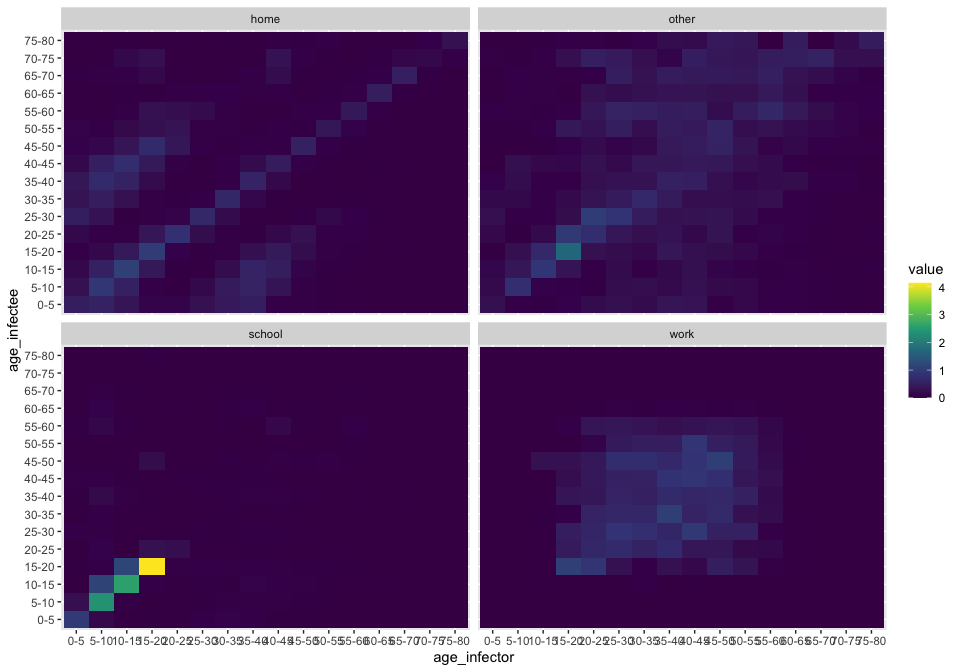
\includegraphics{SEIRD_contact_matrix_files/figure-latex/unnamed-chunk-3-1.pdf}

The availability of contact matrices for different locations facilitates
simulation of age-structured transmission models across geographies. The
current set of age-structured models in \texttt{comomodels} do not
include location-specific infections. Thus, we obtain a single contact
matrix for the age-structured models by summing the four
location-specific contact matrices:

\[
C_{i,j} = C_{i,j}^{\text{home}} + C_{i,j}^{\text{school}} + C_{i,j}^{\text{work}} + C_{i,j}^{\text{other}}.
\] It is possible, however, to investigate how changes to contacts
occurring at a particular class of location affects outputs: simply by
perturbing a particular contact matrix in the above sum.

\hypertarget{uncertainty-in-the-contact-matrix}{%
\subsection{Uncertainty in the contact
matrix}\label{uncertainty-in-the-contact-matrix}}

Typically, when performing simulations of the age-structured SEIRD
model, or inference for the parameters of the model, the contact matrix
is provided as a fixed input. But using fixed values for the contact
matrix neglects the uncertainty inherent in these model inputs.

The purpose of the remainder of this notebook is to investigate the
sensitivity of the outputs of the age-structured SEIRD model (i.e.~the
\texttt{SEIRDAge} model) to the values of the contact matrix. Using
bootstrap samples to represent the uncertainty in the contact matrix, we
show that there is significant uncertainty in the numbers of infected
individuals. The bootstrap algorithm works by selecting a random sample
(with replacement) of the survey respondents, which it then uses to
construct a contact matrix. Across many such samples, the set of contact
matrices provides a measure of uncertainty in the number of daily
contacts across different age groups.

\hypertarget{accuracy-of-uncertainty-estimates-produced-by-the-bootstrapping-methods}{%
\subsection{Accuracy of uncertainty estimates produced by the
bootstrapping
methods}\label{accuracy-of-uncertainty-estimates-produced-by-the-bootstrapping-methods}}

The bootstrap algorithm provides an estimate of contact matrix
uncertainty. There are a range of factors which this approach to
uncertainty quantification does not consider, however. The algorithm
assumes that the original survey from which the contact matrices are
calculated is representative of the underlying population, which may not
be true. For example, if contact data are collected primarily from an
urban area in a country whose population is mostly rural, the resulting
contact matrices would likely be unrepresentative of the country as a
whole. (Indeed, if the two contact matrices differ so markedly, it may
be preferable to model the urban and rural populations separately, as in
the \texttt{SEIRD\_RU} model.) The bootstrap algorithm does not allow
for such biases in quantifying uncertainty, so likely understates true
uncertainty.

\hypertarget{bootstrap-samples-of-contact-matrices}{%
\subsection{Bootstrap samples of contact
matrices}\label{bootstrap-samples-of-contact-matrices}}

We obtain bootstrapped samples of the contact matrix using the
\texttt{socialmixr} library which accesses the POLYMOD data Mossong et
al. (2017). We base our analysis on the UK and generate 200 contact
matrix draws to represent its uncertainty.

\begin{Shaded}
\begin{Highlighting}[]
\CommentTok{\# Define age groups and names}
\NormalTok{ages }\OtherTok{\textless{}{-}} \FunctionTok{seq}\NormalTok{(}\DecValTok{0}\NormalTok{, }\DecValTok{120}\NormalTok{, }\DecValTok{5}\NormalTok{)}
\NormalTok{age\_names }\OtherTok{\textless{}{-}} \FunctionTok{vector}\NormalTok{(}\AttributeTok{length =} \DecValTok{16}\NormalTok{)}
\ControlFlowTok{for}\NormalTok{(i }\ControlFlowTok{in} \FunctionTok{seq\_along}\NormalTok{(age\_names)) \{}
\NormalTok{  age\_names[i] }\OtherTok{\textless{}{-}} \FunctionTok{paste0}\NormalTok{(ages[i], }\StringTok{"{-}"}\NormalTok{, ages[i }\SpecialCharTok{+} \DecValTok{1}\NormalTok{])}
\NormalTok{\}}

\CommentTok{\# Get population data: merge ages 75+}
\NormalTok{pops }\OtherTok{\textless{}{-}}\NormalTok{ population[population}\SpecialCharTok{$}\NormalTok{country }\SpecialCharTok{==} \StringTok{"United Kingdom"}\NormalTok{, ]}\SpecialCharTok{$}\NormalTok{pop}
\NormalTok{pop\_fraction }\OtherTok{\textless{}{-}}\NormalTok{ pops }\SpecialCharTok{/} \FunctionTok{sum}\NormalTok{(pops)}
\NormalTok{pop\_fraction[}\DecValTok{16}\NormalTok{] }\OtherTok{\textless{}{-}} \FunctionTok{sum}\NormalTok{(pop\_fraction[}\DecValTok{16}\SpecialCharTok{:}\DecValTok{21}\NormalTok{])}
\NormalTok{pop\_fraction }\OtherTok{\textless{}{-}}\NormalTok{ pop\_fraction[}\DecValTok{1}\SpecialCharTok{:}\DecValTok{16}\NormalTok{]}
\NormalTok{n\_ages }\OtherTok{\textless{}{-}} \DecValTok{16}

\CommentTok{\# Load the contact matrix data from POLYMOD and get bootstrap samples}
\NormalTok{n\_bootstrap }\OtherTok{\textless{}{-}} \DecValTok{10}
\FunctionTok{data}\NormalTok{(polymod)}
\NormalTok{polymod\_data }\OtherTok{\textless{}{-}} \FunctionTok{contact\_matrix}\NormalTok{(polymod,}
                               \AttributeTok{n=}\NormalTok{n\_bootstrap,}
                               \AttributeTok{countries=}\StringTok{"United Kingdom"}\NormalTok{,}
                               \AttributeTok{age.limits=}\NormalTok{ages)}

\CommentTok{\# Get the first element of the list, which contains the matrices}
\CommentTok{\# In general, bootstrap sampling fails for the 80+ age group,}
\CommentTok{\# so we assume contact patterns remain same as for 75{-}80 y.o.s}
\NormalTok{matrices }\OtherTok{\textless{}{-}}\NormalTok{ polymod\_data[}\StringTok{"matrices"}\NormalTok{][[}\DecValTok{1}\NormalTok{]]}
\end{Highlighting}
\end{Shaded}

First, we inspect the range of values in the sampled contact matrices.
In the plot below, we show the variation in within-age-group daily
contacts: i.e.~we plot the samples of the diagonal elements of the
contact matrix.

\begin{Shaded}
\begin{Highlighting}[]
\NormalTok{contacts\_same\_age }\OtherTok{\textless{}{-}} \FunctionTok{c}\NormalTok{()}
\NormalTok{ages\_list }\OtherTok{\textless{}{-}} \FunctionTok{c}\NormalTok{()}
\ControlFlowTok{for}\NormalTok{ (i }\ControlFlowTok{in} \DecValTok{1}\SpecialCharTok{:}\NormalTok{n\_bootstrap)\{}
\NormalTok{  diags }\OtherTok{\textless{}{-}} \FunctionTok{diag}\NormalTok{(matrices[[i]][[}\DecValTok{1}\NormalTok{]])[}\DecValTok{1}\SpecialCharTok{:}\DecValTok{16}\NormalTok{]}
\NormalTok{  contacts\_same\_age }\OtherTok{\textless{}{-}} \FunctionTok{append}\NormalTok{(contacts\_same\_age,}
\NormalTok{                              diags)}
\NormalTok{  ages\_list }\OtherTok{\textless{}{-}} \FunctionTok{append}\NormalTok{(ages\_list, age\_names)}
\NormalTok{\}}

\NormalTok{data }\OtherTok{\textless{}{-}} \FunctionTok{data.frame}\NormalTok{(ages\_list, contacts\_same\_age)}
\NormalTok{data}\SpecialCharTok{$}\NormalTok{ages\_list }\OtherTok{\textless{}{-}} \FunctionTok{factor}\NormalTok{(data}\SpecialCharTok{$}\NormalTok{ages\_list, }\AttributeTok{levels=}\NormalTok{age\_names[}\DecValTok{1}\SpecialCharTok{:}\DecValTok{16}\NormalTok{], }\AttributeTok{ordered=}\ConstantTok{TRUE}\NormalTok{)}

\FunctionTok{ggplot}\NormalTok{(data, }\FunctionTok{aes}\NormalTok{(}\AttributeTok{x=}\NormalTok{ages\_list, }\AttributeTok{y=}\NormalTok{contacts\_same\_age)) }\SpecialCharTok{+}
  \FunctionTok{geom\_boxplot}\NormalTok{() }\SpecialCharTok{+}
  \FunctionTok{xlab}\NormalTok{(}\StringTok{"age group"}\NormalTok{) }\SpecialCharTok{+}
  \FunctionTok{ylab}\NormalTok{(}\StringTok{"number of daily within{-}group contacts"}\NormalTok{)}
\end{Highlighting}
\end{Shaded}

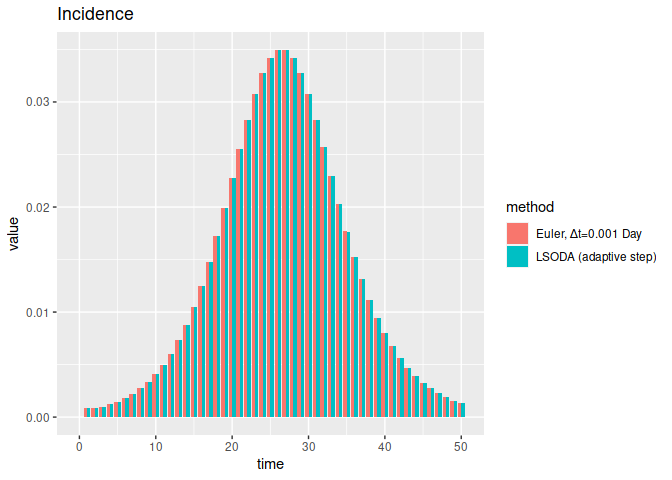
\includegraphics{SEIRD_contact_matrix_files/figure-latex/unnamed-chunk-5-1.pdf}

The plot shows that ages 5--20 (i.e.~mostly school children) have the
greatest possible variation in contacts. Most likely, this is because
this age group has the most contacts.

\hypertarget{the-influence-of-contact-matrix-uncertainty-on-epidemic-dynamics}{%
\subsection{The influence of contact matrix uncertainty on epidemic
dynamics}\label{the-influence-of-contact-matrix-uncertainty-on-epidemic-dynamics}}

To explore the sensitivity of model output to the entries in the contact
matrix, we run the age-structured SEIRD model once for each bootstrap
sample of the contact matrix. We use fixed values for the other
parameters of the model. Initially, we assume that 0.1\% of the
population has been exposed to infection, with the remainder of the
population susceptible.

Here, we assume the transmission dynamics are representative of
ancestral SARS-CoV-2 and obtain representative values from the
\texttt{covid\_transmission\_parameters()} function in
\texttt{comomodels}. For further details on these chosen parameter
values, we refer the interested reader to this function's documentation.

\begin{Shaded}
\begin{Highlighting}[]
\CommentTok{\# Age structured parameters}
\NormalTok{mu }\OtherTok{\textless{}{-}} \FunctionTok{covid\_transmission\_parameters}\NormalTok{(}\AttributeTok{is\_age\_structured=}\ConstantTok{TRUE}\NormalTok{)[}\DecValTok{4}\NormalTok{]}\SpecialCharTok{$}\NormalTok{mu}\SpecialCharTok{$}\NormalTok{mu[}\DecValTok{1}\SpecialCharTok{:}\DecValTok{8}\NormalTok{]}
\NormalTok{mu\_age\_vals }\OtherTok{\textless{}{-}} \FunctionTok{rep}\NormalTok{(mu, }\AttributeTok{each=}\DecValTok{2}\NormalTok{)}

\NormalTok{gamma }\OtherTok{\textless{}{-}} \FunctionTok{covid\_transmission\_parameters}\NormalTok{(}\AttributeTok{is\_age\_structured=}\ConstantTok{TRUE}\NormalTok{)[}\DecValTok{3}\NormalTok{]}\SpecialCharTok{$}\NormalTok{gamma}\SpecialCharTok{$}\NormalTok{gamma[}\DecValTok{1}\SpecialCharTok{:}\DecValTok{8}\NormalTok{]}
\NormalTok{gamma\_age\_vals }\OtherTok{\textless{}{-}} \FunctionTok{rep}\NormalTok{(gamma, }\AttributeTok{each=}\DecValTok{2}\NormalTok{)}

\CommentTok{\# Set the non{-}age structured parameters}
\NormalTok{parameters }\OtherTok{\textless{}{-}} \FunctionTok{covid\_transmission\_parameters}\NormalTok{()}
\NormalTok{kappa }\OtherTok{\textless{}{-}}\NormalTok{ parameters}\SpecialCharTok{$}\NormalTok{kappa}
\NormalTok{gamma }\OtherTok{\textless{}{-}}\NormalTok{ parameters}\SpecialCharTok{$}\NormalTok{gamma}
\NormalTok{mu }\OtherTok{\textless{}{-}}\NormalTok{ parameters}\SpecialCharTok{$}\NormalTok{mu}
\NormalTok{R0\_target }\OtherTok{\textless{}{-}}\NormalTok{ parameters}\SpecialCharTok{$}\NormalTok{R0}
\NormalTok{beta }\OtherTok{\textless{}{-}}\NormalTok{ (mu }\SpecialCharTok{+}\NormalTok{ gamma) }\SpecialCharTok{*}\NormalTok{ R0\_target}
\end{Highlighting}
\end{Shaded}

With the parameter values set, we now simulate the \texttt{SEIRDAge}
model for one year for each of the bootstrap samples of the contact
matrix.

\begin{Shaded}
\begin{Highlighting}[]
\NormalTok{times }\OtherTok{\textless{}{-}} \FunctionTok{seq}\NormalTok{(}\DecValTok{0}\NormalTok{, }\DecValTok{365}\NormalTok{, }\AttributeTok{by=}\DecValTok{1}\NormalTok{)}
\ControlFlowTok{for}\NormalTok{ (i }\ControlFlowTok{in} \DecValTok{1}\SpecialCharTok{:}\NormalTok{n\_bootstrap)\{}
\NormalTok{  matrix}\OtherTok{=}\NormalTok{matrices[[i]][[}\DecValTok{1}\NormalTok{]]}

  \CommentTok{\# Remove the column and row names so the model will accept it}
  \FunctionTok{colnames}\NormalTok{(matrix) }\OtherTok{\textless{}{-}} \ConstantTok{NULL}
  \FunctionTok{rownames}\NormalTok{(matrix) }\OtherTok{\textless{}{-}} \ConstantTok{NULL}

  \CommentTok{\# Keep the data for ages 0{-}80, in 5 year increments}
\NormalTok{  matrix }\OtherTok{\textless{}{-}}\NormalTok{ matrix[}\DecValTok{1}\SpecialCharTok{:}\DecValTok{16}\NormalTok{, }\DecValTok{1}\SpecialCharTok{:}\DecValTok{16}\NormalTok{]}

\NormalTok{  model }\OtherTok{\textless{}{-}}\NormalTok{ comomodels}\SpecialCharTok{::}\FunctionTok{SEIRDAge}\NormalTok{(}\AttributeTok{n\_age\_categories=}\NormalTok{n\_ages,}
                   \AttributeTok{contact\_matrix=}\NormalTok{matrix,}
                   \AttributeTok{age\_ranges=}\FunctionTok{as.list}\NormalTok{(age\_names))}

  \CommentTok{\# Set the other parameters of the model}
  \FunctionTok{transmission\_parameters}\NormalTok{(model) }\OtherTok{\textless{}{-}} \FunctionTok{list}\NormalTok{(}\AttributeTok{b=}\NormalTok{beta,}
                                         \AttributeTok{k=}\NormalTok{kappa,}
                                         \AttributeTok{g=}\NormalTok{gamma\_age\_vals,}
                                         \AttributeTok{mu=}\NormalTok{mu\_age\_vals)}

  \FunctionTok{initial\_conditions}\NormalTok{(model) }\OtherTok{\textless{}{-}} \FunctionTok{list}\NormalTok{(}\AttributeTok{S0=}\NormalTok{pop\_fraction}\SpecialCharTok{*}\FloatTok{0.999}\NormalTok{,}
                                    \AttributeTok{E0=}\FunctionTok{rep}\NormalTok{(}\DecValTok{0}\NormalTok{, n\_ages),}
                                    \AttributeTok{I0=}\NormalTok{pop\_fraction}\SpecialCharTok{*}\FloatTok{0.001}\NormalTok{,}
                                    \AttributeTok{R0=}\FunctionTok{rep}\NormalTok{(}\DecValTok{0}\NormalTok{, n\_ages),}
                                    \AttributeTok{D0=}\FunctionTok{rep}\NormalTok{(}\DecValTok{0}\NormalTok{, n\_ages))}
  
  \CommentTok{\# Run model}
\NormalTok{  res }\OtherTok{\textless{}{-}} \FunctionTok{run}\NormalTok{(model, }\AttributeTok{time=}\NormalTok{times)}
  
  \CommentTok{\# Get states from results}
\NormalTok{  res }\OtherTok{\textless{}{-}}\NormalTok{ res}\SpecialCharTok{$}\NormalTok{states}

  \CommentTok{\# Save the data for the I and R compartments}
\NormalTok{  x }\OtherTok{\textless{}{-}}\NormalTok{ res }\SpecialCharTok{\%\textgreater{}\%}
    \FunctionTok{filter}\NormalTok{(compartment }\SpecialCharTok{\%in\%} \FunctionTok{c}\NormalTok{(}\StringTok{"I"}\NormalTok{, }\StringTok{"R"}\NormalTok{, }\StringTok{"D"}\NormalTok{)) }\SpecialCharTok{\%\textgreater{}\%} 
    \FunctionTok{mutate}\NormalTok{(}\AttributeTok{iteration=}\NormalTok{i)}
  \ControlFlowTok{if}\NormalTok{ (i }\SpecialCharTok{==} \DecValTok{1}\NormalTok{)}
\NormalTok{    all\_results }\OtherTok{\textless{}{-}}\NormalTok{ x}
  \ControlFlowTok{else}
\NormalTok{    all\_results }\OtherTok{\textless{}{-}} \FunctionTok{rbind}\NormalTok{(all\_results, x)}
\NormalTok{\}}
\end{Highlighting}
\end{Shaded}

We then use the simulations to generate the central 90\% quantiles in
the infectious population size for two age groups: 15-20 year olds and
75-80 year olds. We plot these quantiles below.

\begin{Shaded}
\begin{Highlighting}[]
\CommentTok{\# Filter and find quantiles}
\NormalTok{I\_df }\OtherTok{\textless{}{-}}\NormalTok{ all\_results }\SpecialCharTok{\%\textgreater{}\%}
  \FunctionTok{filter}\NormalTok{(age\_range }\SpecialCharTok{\%in\%} \FunctionTok{c}\NormalTok{(}\StringTok{"15{-}20"}\NormalTok{, }\StringTok{"75{-}80"}\NormalTok{),}
\NormalTok{         compartment}\SpecialCharTok{==}\StringTok{"I"}\NormalTok{) }\SpecialCharTok{\%\textgreater{}\%} 
  \FunctionTok{mutate}\NormalTok{(}\AttributeTok{value=}\NormalTok{value }\SpecialCharTok{*} \FunctionTok{sum}\NormalTok{(pops)) }\SpecialCharTok{\%\textgreater{}\%} 
  \FunctionTok{group\_by}\NormalTok{(time, age\_range) }\SpecialCharTok{\%\textgreater{}\%} 
  \FunctionTok{summarise}\NormalTok{(}\AttributeTok{lower=}\FunctionTok{quantile}\NormalTok{(value, }\FloatTok{0.05}\NormalTok{),}
            \AttributeTok{middle=}\FunctionTok{quantile}\NormalTok{(value, }\FloatTok{0.5}\NormalTok{),}
            \AttributeTok{upper=}\FunctionTok{quantile}\NormalTok{(value, }\FloatTok{0.95}\NormalTok{))}

\CommentTok{\# Plot}
\FunctionTok{ggplot}\NormalTok{(I\_df, }\FunctionTok{aes}\NormalTok{(}\AttributeTok{x =}\NormalTok{ time)) }\SpecialCharTok{+}
  \FunctionTok{geom\_ribbon}\NormalTok{(}\FunctionTok{aes}\NormalTok{(}\AttributeTok{ymin =}\NormalTok{ lower, }\AttributeTok{ymax =}\NormalTok{ upper),}
              \AttributeTok{fill =} \StringTok{"blue"}\NormalTok{, }\AttributeTok{alpha =} \FloatTok{0.5}\NormalTok{) }\SpecialCharTok{+}
  \FunctionTok{geom\_line}\NormalTok{(}\FunctionTok{aes}\NormalTok{(}\AttributeTok{y =}\NormalTok{ middle)) }\SpecialCharTok{+}
  \FunctionTok{facet\_wrap}\NormalTok{(}\SpecialCharTok{\textasciitilde{}}\NormalTok{age\_range) }\SpecialCharTok{+}
  \FunctionTok{xlab}\NormalTok{(}\StringTok{"time (days)"}\NormalTok{)}
\end{Highlighting}
\end{Shaded}

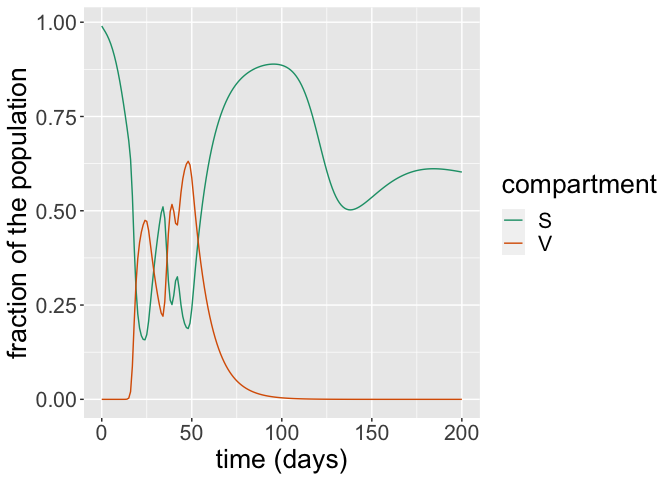
\includegraphics{SEIRD_contact_matrix_files/figure-latex/unnamed-chunk-8-1.pdf}

In both age groups, the results show that there is considerable
uncertainty in the peak infectious counts, but with considerably higher
variation for the older age group -- a result that is particularly
worrying given the greater risk of severe disease facaed by older
individuals (Verity et al. 2020).

Next, we examine the proportion of individuals infected with COVID-19 at
the end of the year, which we plot below. Here, we consider only those
individuals who have survived infection.

\begin{Shaded}
\begin{Highlighting}[]
\CommentTok{\# Filter data}
\NormalTok{df }\OtherTok{\textless{}{-}}\NormalTok{ all\_results }\SpecialCharTok{\%\textgreater{}\%}
  \FunctionTok{filter}\NormalTok{(compartment }\SpecialCharTok{==} \StringTok{"R"}\NormalTok{) }\SpecialCharTok{\%\textgreater{}\%} 
  \FunctionTok{filter}\NormalTok{(time }\SpecialCharTok{==} \DecValTok{365}\NormalTok{)}

\CommentTok{\# Plot}
\FunctionTok{ggplot}\NormalTok{(df,}
       \FunctionTok{aes}\NormalTok{(}\AttributeTok{x=}\NormalTok{age\_range, }\AttributeTok{y=}\NormalTok{value}\SpecialCharTok{/}\NormalTok{pop\_fraction)) }\SpecialCharTok{+}
  \FunctionTok{geom\_boxplot}\NormalTok{() }\SpecialCharTok{+}
  \FunctionTok{xlab}\NormalTok{(}\StringTok{"age group"}\NormalTok{) }\SpecialCharTok{+}
  \FunctionTok{ylab}\NormalTok{(}\StringTok{"proportion of age group previously infected with COVID{-}19"}\NormalTok{)}
\end{Highlighting}
\end{Shaded}

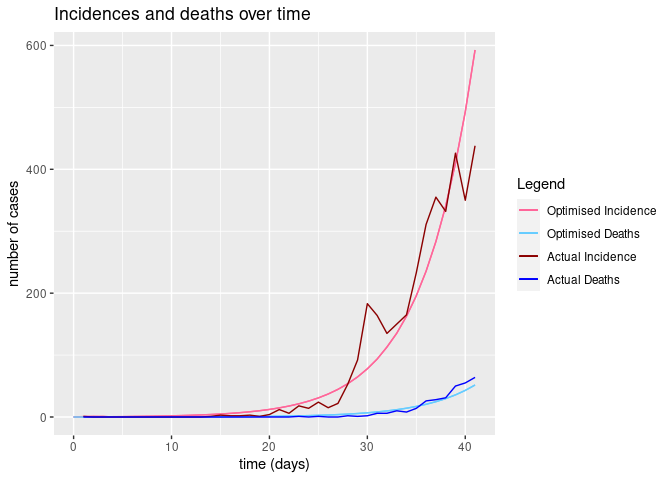
\includegraphics{SEIRD_contact_matrix_files/figure-latex/unnamed-chunk-9-1.pdf}
This plot shows that those aged 5--20 are those most likely to have been
infected by COVID-19: mainly because these individuals have the highest
number of contacts and, because of this, are important drivers of
infections within the population.

This plot also illustrates the pronounced uncertainty in the proportion
of infecteds in the oldest age group.

Finally, we study the effect of uncertainty in the contact matrix on the
number of individuals that die of the infection.

\begin{Shaded}
\begin{Highlighting}[]
\CommentTok{\# Filter dataset}
\NormalTok{df }\OtherTok{\textless{}{-}}\NormalTok{ all\_results }\SpecialCharTok{\%\textgreater{}\%} 
  \FunctionTok{filter}\NormalTok{(compartment }\SpecialCharTok{==} \StringTok{"D"}\NormalTok{) }\SpecialCharTok{\%\textgreater{}\%} 
  \FunctionTok{filter}\NormalTok{(time }\SpecialCharTok{==} \DecValTok{365}\NormalTok{)}

\CommentTok{\# Plot}
\FunctionTok{ggplot}\NormalTok{(df, }\FunctionTok{aes}\NormalTok{(}\AttributeTok{x=}\NormalTok{age\_range, }\AttributeTok{y=}\NormalTok{value }\SpecialCharTok{/}\NormalTok{ pop\_fraction)) }\SpecialCharTok{+}
  \FunctionTok{geom\_boxplot}\NormalTok{() }\SpecialCharTok{+}
  \FunctionTok{xlab}\NormalTok{(}\StringTok{"age group"}\NormalTok{) }\SpecialCharTok{+}
  \FunctionTok{ylab}\NormalTok{(}\StringTok{"proportion of age group dying due to COVID{-}19 infection"}\NormalTok{)}
\end{Highlighting}
\end{Shaded}

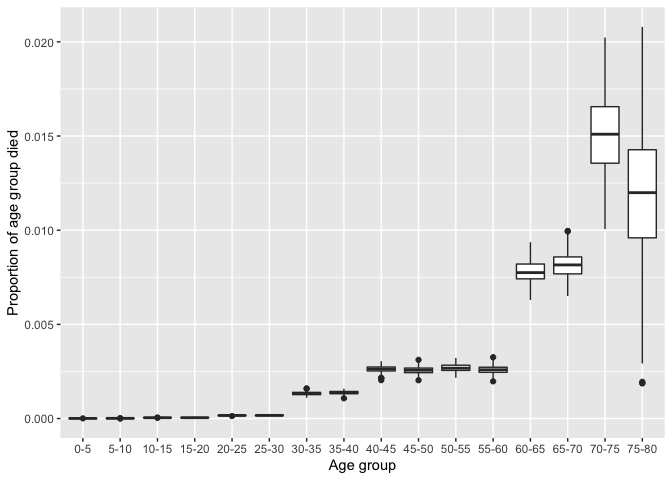
\includegraphics{SEIRD_contact_matrix_files/figure-latex/unnamed-chunk-10-1.pdf}

Although younger people are more likely to be infected due to their
higher number of contacts, deaths occur mainly in the elderly. The
bootstrapped samples of the contact matrix generate a wide range of
deaths, particularly in the oldest age groups.

\hypertarget{conclusion}{%
\subsection{Conclusion}\label{conclusion}}

Who we interact with and how often we interact changes as we age.
COVID-19 is predominantly spread from close contact with infected
individuals and has a strong age-profile of severe disease. Because of
this, mathematical models of disease transmission are often acutely
sensitive to estimates of age-specific contact patterns.

\hypertarget{references}{%
\subsection*{References}\label{references}}
\addcontentsline{toc}{subsection}{References}

\hypertarget{refs}{}
\begin{CSLReferences}{1}{0}
\leavevmode\hypertarget{ref-arregui2018projecting}{}%
Arregui, Sergio, Alberto Aleta, Joaquı́n Sanz, and Yamir Moreno. 2018.
{``Projecting Social Contact Matrices to Different Demographic
Structures.''} \emph{PLOS Computational Biology} 14 (12): e1006638.

\leavevmode\hypertarget{ref-funk2020mixr}{}%
Funk, Sebastian. 2020. \emph{Socialmixr: Social Mixing Matrices for
Infectious Disease Modelling}.
\url{https://CRAN.R-project.org/package=socialmixr}.

\leavevmode\hypertarget{ref-polymod2017}{}%
Mossong, Joel, Niel Hens, Mark Jit, Philippe Beutels, Kari Auranen,
Rafael Mikolajczyk, Marco Massari, et al. 2017. {``POLYMOD Social
Contact Data.''} \emph{Zenodo}.

\leavevmode\hypertarget{ref-prem2021projecting}{}%
Prem, Kiesha, Kevin van Zandvoort, Petra Klepac, Rosalind M Eggo,
Nicholas G Davies, Centre for the Mathematical Modelling of Infectious
Diseases COVID-19 Working Group, Alex R Cook, and Mark Jit. 2021.
{``Projecting Contact Matrices in 177 Geographical Regions: An Update
and Comparison with Empirical Data for the COVID-19 Era.''} \emph{PLOS
Computational Biology} 17 (7): e1009098.

\leavevmode\hypertarget{ref-verity2020estimates}{}%
Verity, Robert, Lucy C Okell, Ilaria Dorigatti, Peter Winskill, Charles
Whittaker, Natsuko Imai, Gina Cuomo-Dannenburg, et al. 2020.
{``Estimates of the Severity of Coronavirus Disease 2019: A Model-Based
Analysis.''} \emph{The Lancet Infectious Diseases} 20 (6): 669--77.

\end{CSLReferences}

\end{document}
